\documentclass[11pt,a4paper]{article}

\usepackage{indentfirst}
\usepackage{amssymb}
\usepackage{subcaption}
\usepackage{graphicx}
\usepackage{longtable}
\usepackage{fancyhdr}
\usepackage{xeCJK}
\usepackage{amsmath}
\usepackage{amssymb}
\usepackage{ulem}
\usepackage{xcolor}
\usepackage{fancyvrb}
\usepackage{listings}
\usepackage{soul}
\usepackage{hyperref}
	\lstdefinestyle{C}{
   		language=C, 
   		basicstyle=\ttfamily\bfseries,
    	numbers=left, 
    	numbersep=5pt,
    	tabsize=4,
    	frame=single,
   	 	commentstyle=\itshape\color{brown},
    	keywordstyle=\bfseries\color{blue},
   	 	deletekeywords={define},
    	morekeywords={NULL,bool}
	}	

\setCJKmainfont{Noto Sans Mono CJK TC}
 
\voffset -20pt
\textwidth 410pt
\textheight 650pt
\oddsidemargin 20pt
\newcommand{\XOR}{\otimes}
\linespread{1.2}\selectfont
\graphicspath{{images/}}

\pagestyle{fancy}
\lhead{國立宜蘭高中 111 學年度資訊學科能力競賽}

\begin{document}

\begin{center}
\section*{E. 妙妙網路城}
\end{center}

\section*{Description}

又到了四年一度的地方首長選戰對決,各地候選人摩拳擦掌,準備角逐百里侯大位。
身為割馬籃共和國首長的妙妙姊也不例外,預計在這最後的時間衝刺建設,以實質的政績求選票、拚連任。
根據妙妙姊的幕僚指出,在現今的 5G 時代,最好的建設就是超讚的網路速度。
因次這次妙妙姊決定聽取建議,為國內各地鋪設大量光纖網路,讓所有居民都能享有高速的上網體驗。

割馬籃共和國是由有 $N$ 座城鎮所組成,其中編號 $1$ 城鎮是政府所在地,亦是網路供應的源頭。
在政府宣傳招商後,若干家廠商總計提供了 $M$ 條光纖建設方案,每條方案包含以下資訊:
\begin{itemize}
	\item $a_i,\ b_i$:代表該方案連接城鎮 $a_i$ 與 城鎮 $b_i$。
	\item $c_i$:代表該方案是來自編號 $c_i$ 廠商。
\end{itemize}

妙妙姊必須選定一些建設方案,使得所有城鎮都能透過數條光纖連接到城鎮 $1$,以便獲取超高速網路。
然而建設這些光纖的費用跟妙妙姊一樣奇妙,或許是編號相近的廠商能更加順利合作的關係,建設費用竟然取決選定的廠商編號全距。
換句話說,若 $S$ 為選定方案的集合,則建設費用 $P$ 為 
$$
	P = \max(c_j) - \min(c_j),\quad c_j \in S
$$
也就是編號最大的廠商減掉編號最小的廠商。

為了割馬籃共和國著想,避免官商勾結,花大錢做小事。
請你幫妙妙姊計算看看,最少需要花費多少建設費用才能將所有城鎮都連接到城鎮 $1$?

\section*{Input}

第一行包含兩個正整數 $N, M$,分別代表城鎮與建設方案數量。

接下來 $M$ 行,每行有三個正整數 $a_i, b_i, c_i$,代表該方案連接城鎮 $a_i$ 與 $b_i$,並且來自編號 $c_i$ 廠商。

各變數範圍限制如下:
\begin{itemize}
    \item $2 \le N \le 10^5$
    \item $1 \le M \le 2\times 10^5$
    \item $1 \le a_i, b_i \le N$
    \item $a_i \neq b_i$
    \item $1 \le c_i \le 100$
    \item 保證所有城鎮必定可以透過數條方案連接到城鎮 $1$
\end{itemize}

\section*{Output}

請輸出一個整數代表最小的建設花費。

\section*{Sample 1}
\begin{longtable}[!h]{|p{0.5\textwidth}|p{0.5\textwidth}|}
\hline
\textbf {Input}	& \textbf {Output} \\
\hline
\parbox[t]{0.5\textwidth} % sample 1
{ \tt
% input
4 5 \\
1 2 1 \\
1 3 3 \\
2 3 2 \\
2 4 3 \\
3 4 4 \\
} &
\parbox[t]{0.5\textwidth}
{ \tt
%output
1 \\
} \\
\hline
\end{longtable}

\section*{Sample 2}
\begin{longtable}[!h]{|p{0.5\textwidth}|p{0.5\textwidth}|}
\hline
\textbf {Input}	& \textbf {Output} \\
\hline
\parbox[t]{0.5\textwidth} % sample 2
{ \tt
% input
9 14 \\
1 2 2 \\
1 4 3 \\
1 5 5 \\
1 7 1 \\
2 3 5 \\
2 4 1 \\
3 5 1 \\
4 7 4 \\
4 8 2 \\
4 9 5 \\
5 6 7 \\
5 7 7 \\
6 7 3 \\
7 8 6 \\
} &
\parbox[t]{0.5\textwidth}
{ \tt
%output
3 \\
} \\
\hline
\end{longtable}

\newpage
\section*{Sample 3}
\begin{longtable}[!h]{|p{0.5\textwidth}|p{0.5\textwidth}|}
\hline
\textbf {Input}	& \textbf {Output} \\
\hline
\parbox[t]{0.5\textwidth} % sample 3
{ \tt
% input
6 11 \\
1 2 1 \\
1 3 1 \\
1 4 1 \\
1 5 1 \\
1 6 1 \\
1 6 2 \\
1 6 3 \\
2 3 3 \\
3 4 4 \\
4 5 5 \\
5 6 6 \\
} &
\parbox[t]{0.5\textwidth}
{ \tt
%output
0 \\
} \\
\hline
\end{longtable}

\section*{配分}

在一個子任務的「測試資料範圍」的敘述中,如果存在沒有提到範圍的變數,則此變數的範圍為 Input 所描述的範圍。

\begin{center}
 \begin{tabular}{||c c c||} 
 \hline
 子任務編號 & 子任務配分 & 測試資料範圍 \\  
 \hline\hline
 0 & 0\% & 範例測資 \\ 
 \hline
 1 & 3\% & $1 \le a_i \le 2$ \\
 \hline
 2 & 9\% & $1 \le a_i \le 10,\ 1 \le M \le 2\times 10^3$ \\
 \hline
 3 & 15\% & $1 \le a_i \le 10,\ 1 \le M \le 2\times 10^4$ \\
 \hline
 4 & 28\% & $1 \le a_i \le 10$ \\
 \hline
 5 & 33\% & $1 \le M \le 2\times 10^4$ \\
 \hline
 6 & 12\% & 無額外限制 \\ 
 \hline
\end{tabular}
\end{center}

\newpage
\section*{Hint}
範例一圖樣如下
\begin{center}
	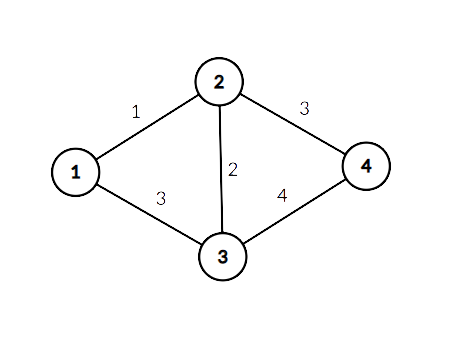
\includegraphics[width=6.5cm]{sample1.png}
\end{center}

範例二圖樣如下
\begin{center}
	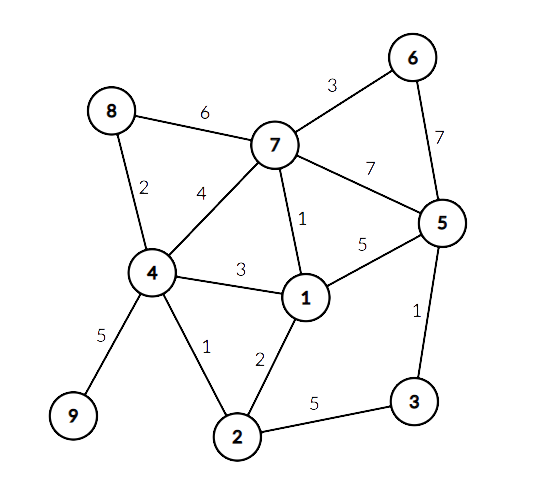
\includegraphics[width=8cm]{sample2.png}
\end{center}

範例三圖樣如下
\begin{center}
	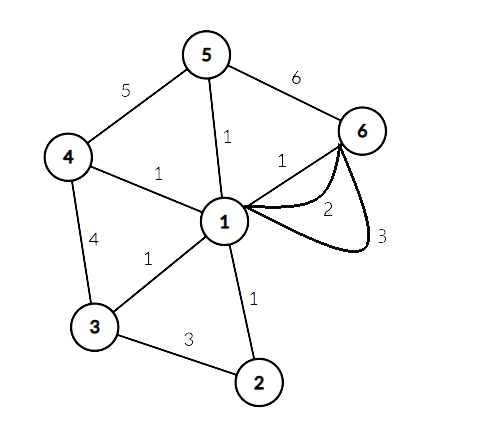
\includegraphics[width=7cm]{sample3.png}
\end{center}



\end{document}
